\documentclass[11pt]{article}
\usepackage{geometry,marginnote} % Pour passer au format A4
\geometry{hmargin=1cm, vmargin=1.5cm} % 

% Page et encodage
\usepackage[T1]{fontenc} % Use 8-bit encoding that has 256 glyphs
\usepackage[english,french]{babel} % Français et anglais
\usepackage[utf8]{inputenc} 

\usepackage{lmodern}
\usepackage[np]{numprint}
\setlength\parindent{0pt}

% Graphiques
\usepackage{graphicx,float,grffile}
\usepackage{tikz,pst-eucl,pst-plot,pstricks,pst-node,pstricks-add,pst-fun,pgfplots} 

% Maths et divers
\usepackage{amsmath,amsfonts,amssymb,amsthm,verbatim,scratch3}
\usepackage{multicol,enumitem,url,eurosym,gensymb,tabularx}

\DeclareUnicodeCharacter{20AC}{\euro}



% Sections
\usepackage{sectsty} % Allows customizing section commands
\allsectionsfont{\centering \normalfont\scshape}

% Tête et pied de page
\usepackage{fancyhdr} \pagestyle{fancy} \fancyhead{} \fancyfoot{}

%\fancyfoot[L]{Collège Faubert}
%\fancyfoot[C]{\thepage / 6}
%\fancyfoot[R]{Série Générale}

\renewcommand{\headrulewidth}{0pt} % Remove header underlines
%\renewcommand{\footrulewidth}{0pt} % Remove footer underlines

\newcommand{\horrule}[1]{\rule{\linewidth}{#1}} % Create horizontal rule command with 1 argument of height

\newcommand{\Pointilles}[1][3]{%
  \multido{}{#1}{\makebox[\linewidth]{\dotfill}\\[\parskip]
}}

\newtheorem{Definition}{Définition}

\usepackage{siunitx}
\sisetup{
    detect-all,
    output-decimal-marker={,},
    group-minimum-digits = 3,
    group-separator={~},
    number-unit-separator={~},
    inter-unit-product={~}
}

\setlength{\columnseprule}{1pt}



\begin{document}



\begin{titlepage}

    \center % Center everything on the page
    
    \textsc{\LARGE Collège Faubert}\\[2cm] % Name of your university/college
    %\textsc{\Large }\\[0.5cm] % Major heading such as course name
    \textsc{\large Villefranche}\\[2cm] % Minor heading such as course title
    
    \horrule{2px}
    
    \vspace{1cm}
    
    { \Huge \bfseries Brevet Blanc}\\[2cm] % Title of your document
    { \Huge \bfseries Mathématiques}\\[2cm] % Title of your document
    {\large \bfseries Février - 2025}\\[2cm] 
    
    \horrule{2px}
    
    \vspace{1cm}
    
    \begin{itemize}[label={$\bullet$}]
      \item \textsc{Exercice 1} - 18 points     
      \item \textsc{Exercice 2} - 20 points 
      \item \textsc{Exercice 3} - 24 points
      \item \textsc{Exercice 4} - 19 points 
      \item \textsc{Exercice 5} - 19 points  
    \end{itemize}
    
    \vspace{1cm}
    
    \horrule{2px}
    
    \vspace{1cm}
    
    \textbf{Le sujet est à rendre avec la copie.}
    
    \vspace{1cm}
    
    \begin{itemize}
      \item L'usage de la calculatrice de type collège est autorisé.
      \item L'usage de tout autre document est interdit. 
      \item L'ensemble des réponses doivent êtres justifiées.
      \item Toute trace écrite, même incomplète sera prise en compte dans l'évaluation.
    \end{itemize}
    
    \vfill 
    
    \end{titlepage}
    
\newpage

\subsection*{Exercice 1 - 18 points }


\subsection*{Exercice 2 - 20 points }

\begin{multicols}{2}\noindent
Programme A

\begin{itemize}[label={$\bullet$}]
  \item Choisir un nombre.
  \item Prendre le carré du nombre choisi.
  \item Multiplier le résultat par 2.
  \item Ajouter le double du nombre de départ. 
  \item Soustraire 4 au résultat.
\end{itemize} \columnbreak


Programme B

\begin{figure}[H]
  \centering
  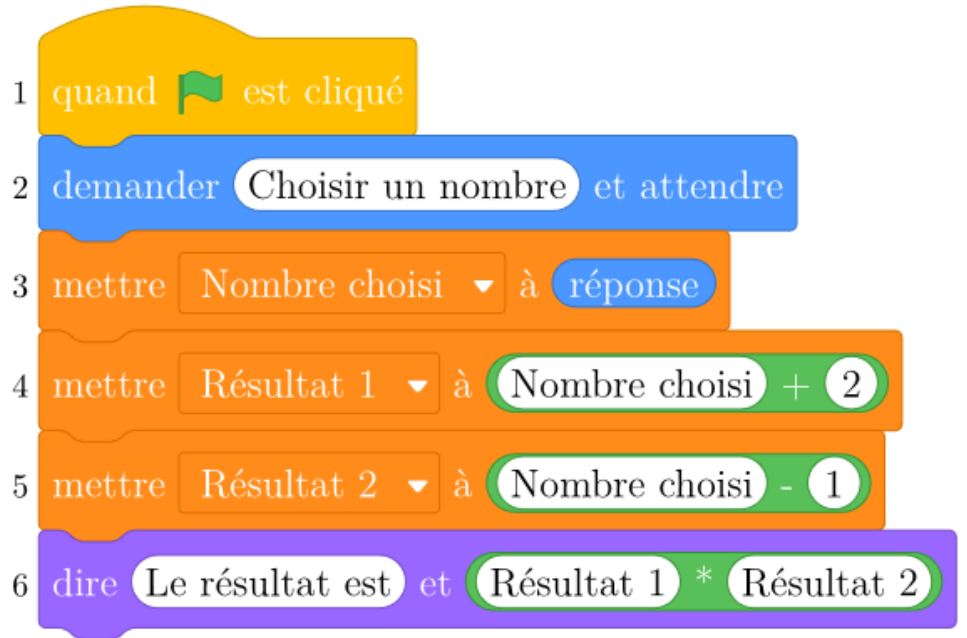
\includegraphics[width=0.8\linewidth]{bb2-ex2.png}
\end{figure}

\end{multicols}




\begin{enumerate}
  \item[1.] 
  \begin{enumerate}
    \item[a.] Vérifier que, si on choisit 5 comme nombre de départ, le résultat du programme A est 56.
    \item[b.] Quel résultat obtient-on avec le programme B si on choisit -9 comme nombre de départ ?
  \end{enumerate} 

  \item[2.] On choisit un nombre quelconque x comme nombre de départ.
  \begin{enumerate}
    \item[a.] Parmi les trois propositions ci-dessous, recopier l'expression qui donne le résultat obtenu par le programme B ?
      
    \begin{multicols}{3}\noindent
      $E_1 = (x+2)-1$ \\
      $E_2 = (x+2) \times (x - 1)$ \\
      $E_3 = x + 2 \times x - 1$ 
    \end{multicols}

    \item[b.] Exprimer en fonction de x le résultat obtenu avec le programme A.
  \end{enumerate} 

  \item[3.] Démontrer que, quel que soit le nombre choisi au départ , le résultat du programme A est toujours le double du résultat du programme B.
\end{enumerate}

\subsection*{Exercice 3 - 24 points }


\subsection*{Exercice 4 - 19 points }


\subsection*{Exercice 5 - 19 points }


\end{document}
